\documentclass[aspectratio=169]{beamer}

\usepackage[utf8]{inputenc}
\usepackage{array}
\usepackage{booktabs}
\usepackage{bold-extra}
\usepackage{graphics}
\usepackage{hyperref}
\hypersetup{%
  colorlinks=true,
  linkcolor=blue,
  filecolor=blue,
  urlcolor=cyan,
}
\usepackage{listings}
\usepackage{multicol}
\usepackage[absolute,overlay]{textpos}
\usepackage{setspace}
\usepackage{verbatim}
\usepackage{fancyvrb} % for verbatim centering
\usepackage{tikz}

\usetheme{Warsaw}
\usecolortheme{beaver}
\definecolor{clOrange}{HTML}{E76600}
\definecolor{clAlmostWhite}{HTML}{FEFFD9}
\definecolor{clGreen}{HTML}{007F00}
\definecolor{clFlag}{HTML}{D33682}
\definecolor{clFlagOpt}{HTML}{CB4B16}
\definecolor{clRedFlag}{HTML}{DC322F}
\definecolor{clGreenFlag}{HTML}{859900}
\definecolor{clViolet}{HTML}{4c0070}
\definecolor{clGray}{HTML}{607060}

\definecolor{clCodeBlue}{rgb}{0.0, 0.18, 0.38}
\definecolor{clCodeGreen}{rgb}{0.0, 0.27, 0.15}
\definecolor{clCodeRed}{rgb}{0.63, 0.0, 0.0}


\setbeamertemplate{navigation symbols}{}
\setbeamercolor{title}{fg=black}
\setbeamercolor{author}{fg=clAlmostWhite}
\setbeamercolor{date}{fg=clAlmostWhite}
\setbeamerfont{author}{size=\huge}
\setbeamerfont{date}{size=\Large}

\newcommand{\greenemph}[1]{\textit{\textcolor{clGreen}{#1}}}
\newcommand{\cpp}[1]{\texttt{\textbf{\textcolor{clCodeBlue}{#1}}}}

\newcommand\fontV{\fontsize{5}{5}\selectfont}
\newcommand\addsource[1]{\fontV\textcolor{clGray}{#1}}

\lstset{
  language=C++,
  basicstyle=\ttfamily,
  keywordstyle=\color{clCodeBlue}\ttfamily,
  stringstyle=\color{clCodeGreen}\ttfamily,
  commentstyle=\color{clCodeRed}\ttfamily,
  morecomment=[l][\color{magenta}]{\#}
}

\title[%
\texttt{\textcolor{clGray}{C++ Friends} %
\textcolor{clCodeBlue}{\#20}\textcolor{clGray}{~::~}\textcolor{clCodeBlue}{EfficiencyOfContainers}}%
]{%
Efficiency of C++ containers%
}
\author{gralin.ski}
\date{May 2022}

\begin{document}

{\usebackgroundtemplate{%
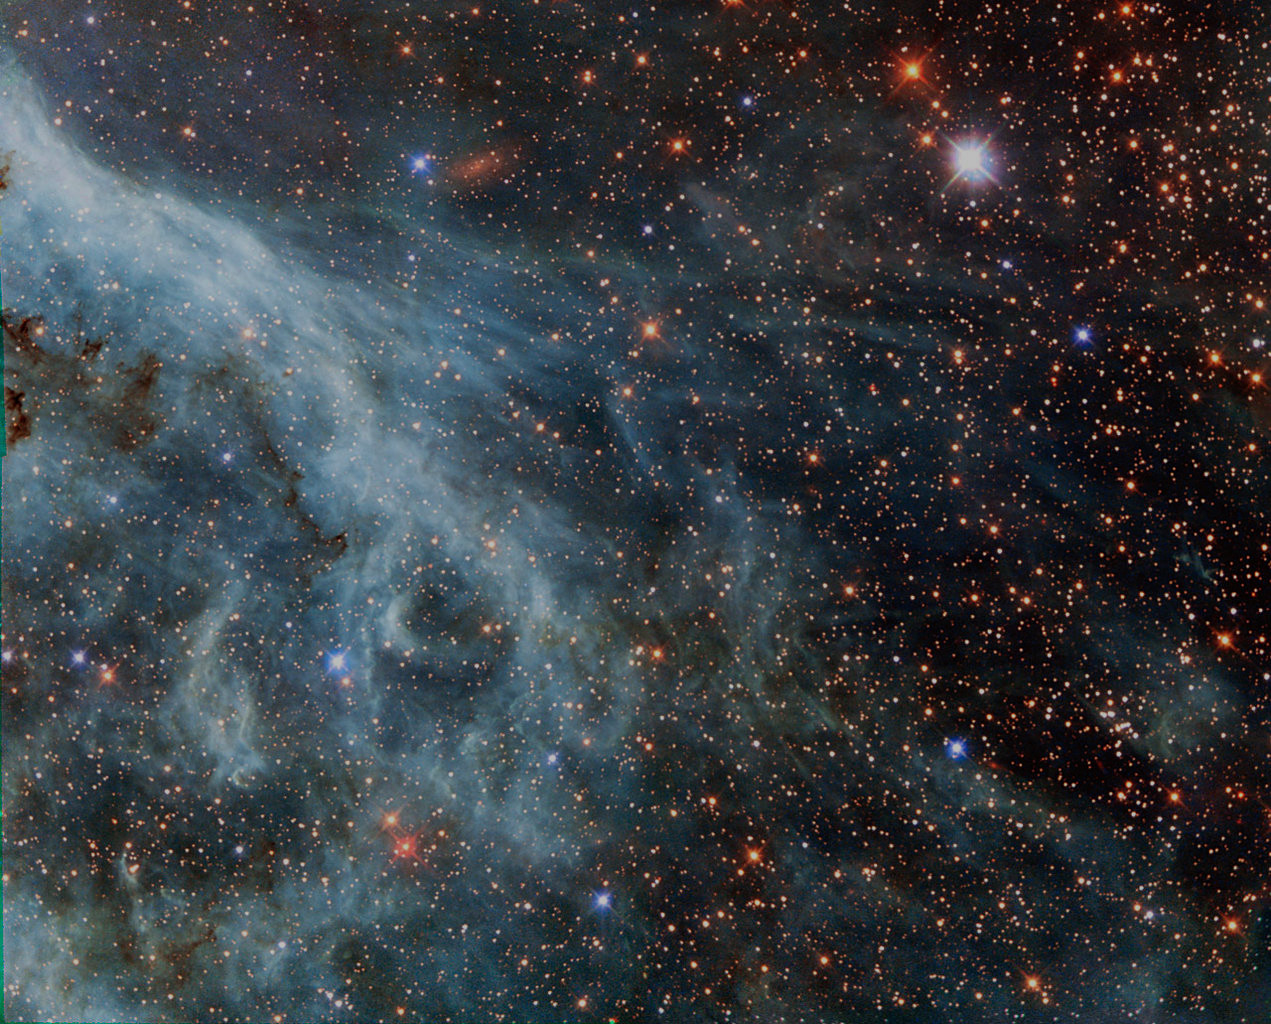
\includegraphics[width=\paperwidth,height=\paperheight]{../../common/bg_galaxy.jpg}}
\begin{frame}
\titlepage{}
\end{frame}
}

\begin{frame}
\frametitle{Efficiency of standard containers}
The standard library provides \textit{containers} to store collections of same type.\\
\vspace*{12pt}
The following containers are \greenemph{dynamic}, meaning that they can grow or shrink\\
as needed --- their size is not fixed.
\vspace*{18pt}
\begin{center}
  \begin{minipage}{0.4\textwidth}
    \begin{itemize}
      \item{} \cpp{std::list}
      \item{} \cpp{std::vector}
      \item{} \cpp{std::deque}
      \item{} \cpp{std::set}
      \item{} \cpp{std::unordered\_set}
    \end{itemize}
  \end{minipage}
\end{center}
\end{frame}

\begin{frame}
\frametitle{Efficiency of standard containers}
\begin{center}
  \begin{minipage}{0.4\textwidth}
    \begin{itemize}
      \item{} \cpp{std::list}
      \item{} \cpp{std::vector}
      \item{} \cpp{std::deque}
      \item{} \cpp{std::set}
      \item{} \cpp{std::unordered\_set}
    \end{itemize}
  \end{minipage}
\end{center}
\vspace*{16pt}
Do you know how do they \greenemph{store the data internally}?\\
\vspace*{12pt}
Can you tell which one is \greenemph{the most optimal}~~for a given task?
\end{frame}

\begin{frame}
\frametitle{Bit of theory --- \cpp{std::list}}
\begin{columns}
  \begin{column}{0.38\textwidth}
    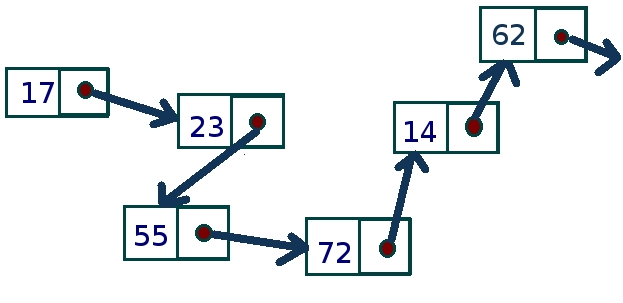
\includegraphics[width=\textwidth]{pictures/Linked_list_layout.jpg} \\
  \end{column}\hfill%
  \begin{column}{0.58\textwidth}
    \begin{tabular}{|l|l|}
      \hline
      Operation & Complexity \\
      \hline\hline
      get(int index) & \textcolor{clRedFlag}{O(n)} \\
      \hline
      push\_back(T element) & O(1) \\
      push\_front(T element) & \\
      \hline
      insert(T element, int index) & \textcolor{clGreenFlag}{O(1)} \\
      \hline
      remove(int index) & O(1) \\
      \hline
    \end{tabular}
  \end{column}
\end{columns}
\vspace*{36pt}
\addsource{image source: a detail of https://commons.wikimedia.org/wiki/File:Linked\_list\_data\_format.jpg}
\end{frame}

\begin{frame}
\frametitle{Bit of theory --- \cpp{std::deque}}
\begin{columns}
  \begin{column}{0.38\textwidth}
    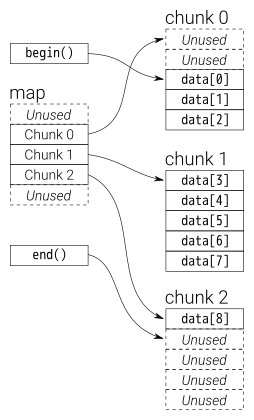
\includegraphics[width=0.6\textwidth]{pictures/deque_layout.png} \\
  \end{column}\hfill%
  \begin{column}{0.58\textwidth}
    \begin{tabular}{|l|l|}
      \hline
      Operation & Complexity \\
      \hline\hline
      get(int index) & O(1) \\
      \hline
      push\_back(T element) & O(1) \\
      push\_front(T element) & \\
      \hline
      insert(T element, int index) & \textcolor{clRedFlag}{O(n)} \\
      \hline
      remove(int index) & \textcolor{clRedFlag}{O(n)} \\
      \hline
    \end{tabular} \\
    \textcolor{clGreenFlag}{O(1)} insert and remove at both ends of deque
  \end{column}
\end{columns}
\vspace*{24pt}
{\centering Note: data is not stored contiguously.\\}
\vspace*{12pt}
\addsource{image source: part of https://stackoverflow.com/questions/6292332/what-really-is-a-deque-in-stl}
\end{frame}

\begin{frame}
\frametitle{Bit of theory --- \cpp{std::vector}}
\begin{columns}
  \begin{column}{0.38\textwidth}
    \includegraphics[width=\textwidth]{pictures/vector_layout.png} \\
  \end{column}\hfill%
  \begin{column}{0.58\textwidth}
    \begin{tabular}{|l|l|}
      \hline
      Operation & Complexity \\
      \hline\hline
      get(int index) & O(1) \\
      \hline
      push\_back(T element) & O(1), may be worse \\
      push\_front(T element) & \textcolor{clRedFlag}{O(n)} \\
      \hline
      insert(T element, int index) & \textcolor{clRedFlag}{O(n)} \\
      \hline
      remove\_back & O(1) \\
      remove(int index) & \textcolor{clRedFlag}{O(n)} \\
      \hline
    \end{tabular} \\
  \end{column}
\end{columns}
\vspace*{24pt}
{\centering Note: data is \textcolor{clGreenFlag}{stored contiguously}.\\}
\vspace*{12pt}
\addsource{image source: part of https://stackoverflow.com/questions/52330010/what-does-stdvector-look-like-in-memory}
\end{frame}

\begin{frame}
\frametitle{Bit of theory --- \cpp{std::set}}
\begin{columns}
  \begin{column}{0.38\textwidth}
    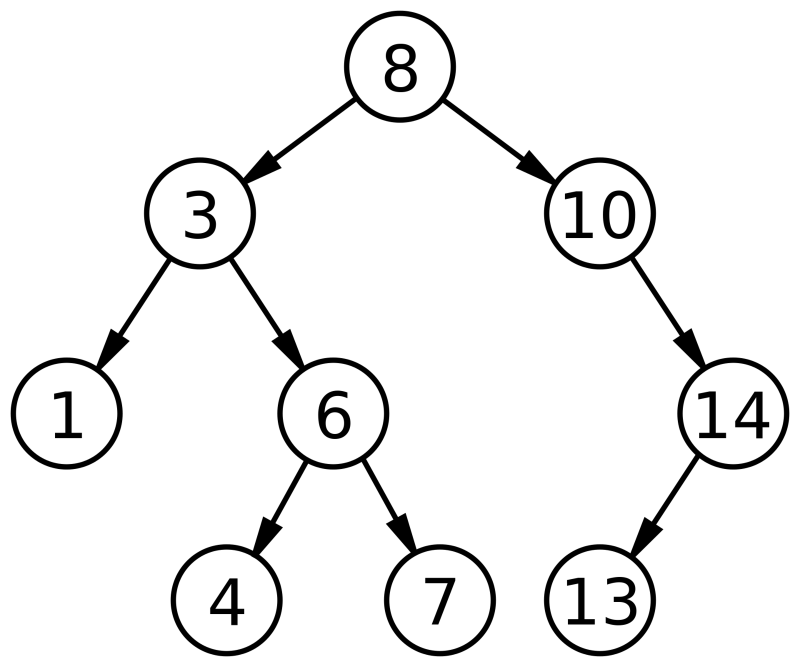
\includegraphics[width=0.8\textwidth]{pictures/bst.png} \\
  \end{column}\hfill%
  \begin{column}{0.58\textwidth}
    \begin{tabular}{|l|l|}
      \hline
      Operation & Complexity \\
      \hline\hline
      get(int index) & \emph{not provided} \\
      \hline
      find(T element) & O(log(n)) \\
      \hline
      insert(T element) & O(log(n)) \\
      \hline
      remove(T element) & O(log(n)) \\
      \hline
    \end{tabular} \\
  \end{column}
\end{columns}
\vspace*{12pt}
{\hspace{3cm} Note [1]: sequential access is not supported.\\}
{\hspace{3cm} Note [2]: uses a \greenemph{binary search tree}.\\}
\vspace*{12pt}
\addsource{image source: part of https://en.wikipedia.org/wiki/Binary\_search\_tree}
\end{frame}


\begin{frame}
\frametitle{Bit of theory --- \cpp{std::unordered\_set}}
\begin{columns}
  \begin{column}{0.38\textwidth}
    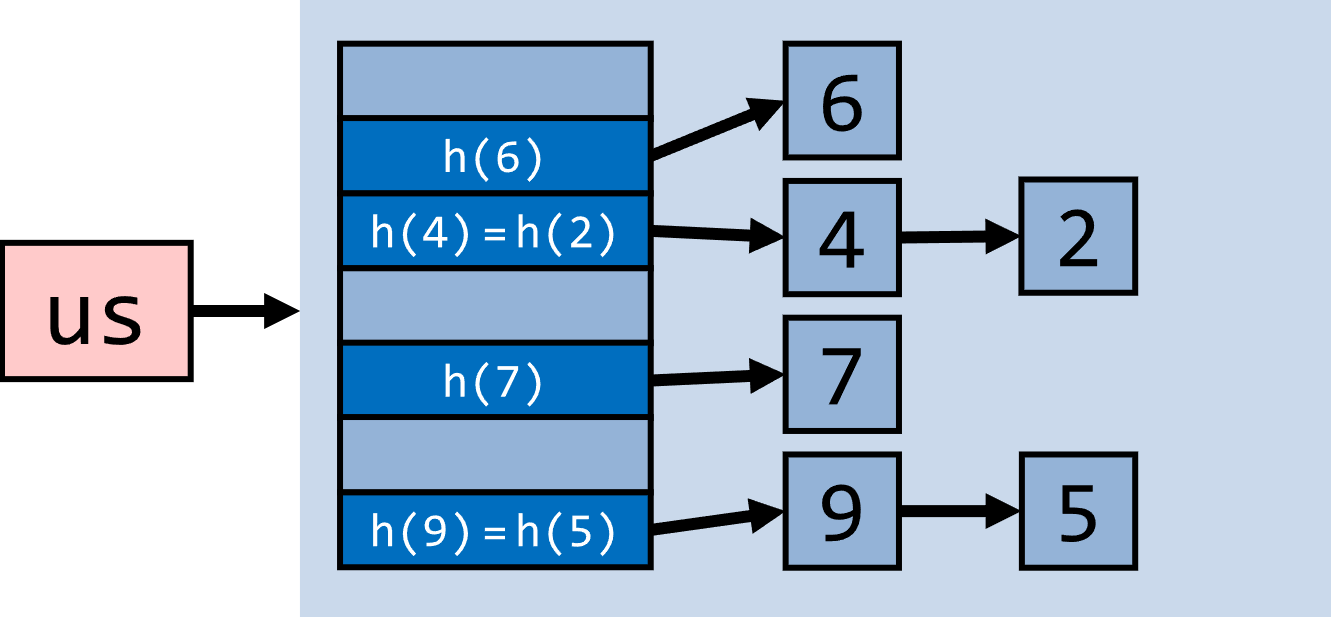
\includegraphics[width=\textwidth]{pictures/unordered_set.png} \\
  \end{column}\hfill%
  \begin{column}{0.58\textwidth}
    \begin{tabular}{|l|l|}
      \hline
      Operation & Complexity \\
      \hline\hline
      get(int index) & \emph{not provided} \\
      \hline
      find(T element) & O(1) or O(n) \\
      \hline
      insert(T element) & O(1) or O(n) \\
      \hline
      remove(T element) & O(1) or O(n) \\
      \hline
    \end{tabular}\\
  \end{column}
\end{columns}
\vspace*{24pt}
{\hspace{1cm}Note: all operation take average \textcolor{clGreenFlag}{O(1) time}.\\}
{\hspace{1cm}It can go up to O(n) in worst case, but in general they perform well.\\}
{\hspace{1cm}In more precise terms, unordered\_set's operations are \textcolor{clViolet}{amortized O(1)}\\}
\vspace*{24pt}
\addsource{image source: https://hackingcpp.com/cpp/std/unordered\_set\_thumb.svg}
\end{frame}

\begin{frame}
\frametitle{Benchmark --- storage of data}
\begin{center}
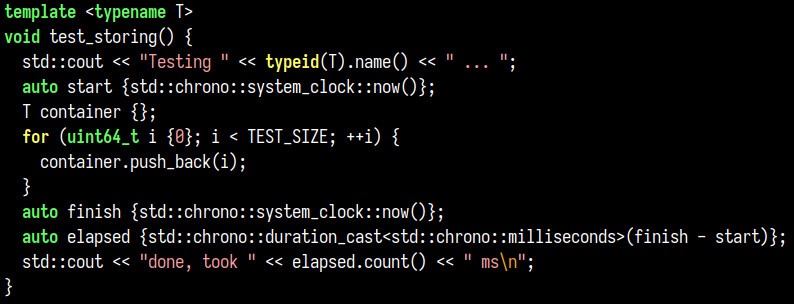
\includegraphics[width=0.5\textwidth]{pictures/code_storing.jpg} \\
\vspace*{16pt}
\begin{tabular}{|l|l|l|l|l|l|}
  \hline
  Trial & \cpp{vector} & \cpp{deque} & \cpp{list} & \cpp{set} & \cpp{unordered\_set} \\
  \hline
  1. & 70 ms & 53 ms & 309 ms & 2745 ms & 761 ms \\
  \hline
  2. & 70 ms & 54 ms & 316 ms & 2667 ms & 730 ms \\
  \hline
  3. & 71 ms & 55 ms & 332 ms & 2700 ms & 769 ms \\
  \hline
\end{tabular}\\
\end{center}
\vspace*{24pt}
\addsource{Tested on an x86\_64 machine with Ryzen 5600X processor. Full code: \cpp{storing.cpp}.}
\end{frame}

\begin{frame}
\frametitle{Benchmark --- accessing data randomly}
\begin{center}
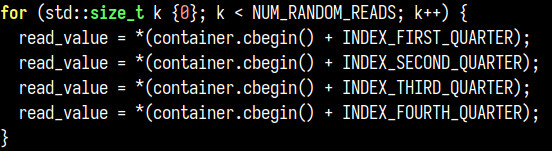
\includegraphics[width=0.5\textwidth]{pictures/code_random_access.jpg}\\
\vspace*{16pt}
\begin{tabular}{|l|l|l|l|l|l|}
  \hline
  Trial & \cpp{vector} & \cpp{deque} & \cpp{list} & \cpp{set} & \cpp{unordered\_set} \\
  \hline
  1. & 150 ms & 304 ms & 2449 ms & 1743 ms & 907 ms \\
  \hline
  2. & 146 ms & 295 ms & 2437 ms & 1754 ms & 902 ms \\
  \hline
  3. & 148 ms & 308 ms & 2446 ms & 1729 ms & 891 ms \\
  \hline
\end{tabular}\\
\end{center}
\vspace*{24pt}
\addsource{Tested on an x86\_64 machine with Ryzen 5600X processor. Full code: \cpp{reading\_random.cpp}.}
\end{frame}

\begin{frame}
\frametitle{Benchmark --- accessing data sequentially}
\begin{center}
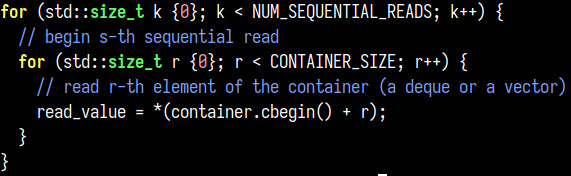
\includegraphics[width=0.5\textwidth]{pictures/code_sequential_access.jpg}\\
\vspace*{16pt}
\begin{tabular}{|l|l|l|l|l|l|}
  \hline
  Trial & \cpp{vector} & \cpp{deque} & \cpp{list} & \cpp{set} & \cpp{unordered\_set} \\
  \hline
  1. & 11 ms & 22 ms & 1357 ms & 143 ms & 45 ms \\
  \hline
  2. & 9 ms & 21 ms & 1353 ms & 145 ms & 45 ms \\
  \hline
  3. & 10 ms & 21 ms & 1360 ms & 143 ms & 45 ms \\
  \hline
\end{tabular}\\
\end{center}
\vspace*{24pt}
\addsource{Tested on an x86\_64 machine with Ryzen 5600X processor. Full code: \cpp{reading\_sequential.cpp}.}
\end{frame}

\begin{frame}
\frametitle{Benchmark --- \cpp{std::vector} or \cpp{std::unordered\_set}?}
\begin{center}
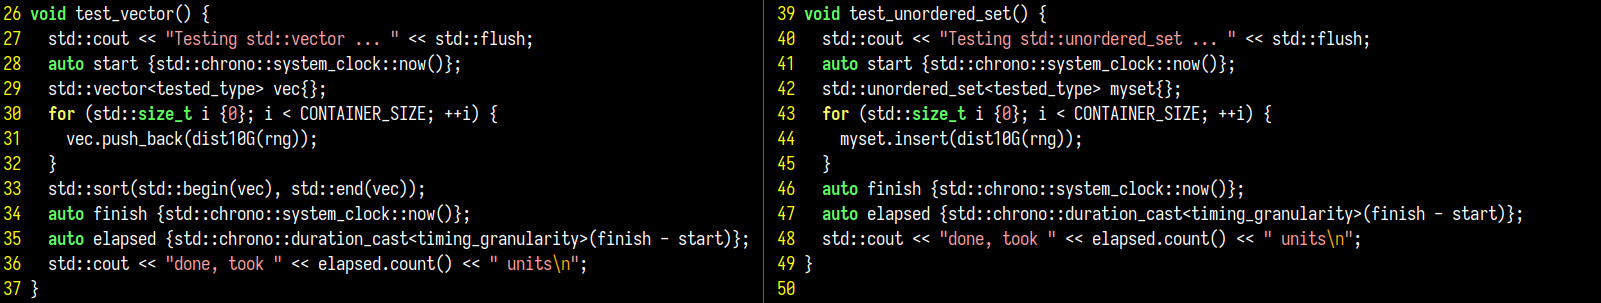
\includegraphics[width=0.8\textwidth]{pictures/code_versus.jpg}\\
\vspace*{16pt}
\begin{tabular}{|l|l|l|}
  \hline
  Container size & \cpp{vector} & \cpp{unordered\_set} \\
  \hline
  10 & $15 \: \mu{}s$ & $7 \: \mu{}s$\\
  \hline
  100 & $23 \: \mu{}s$ & $22 \: \mu{}s$\\
  \hline
  1000 & $251 \: \mu{}s$ & $241 \: \mu{}s$\\
  \hline
  10K & $3834 \: \mu{}s$ & $2659 \: \mu{}s$\\
  \hline
  1M & $374 \: ms$ & $426 \: ms$\\
  \hline
  10M & $4152 \: ms$ & $6109 \: ms$\\
  \hline
\end{tabular}\\
\end{center}
\vspace*{6pt}
\addsource{Tested on an x86\_64 machine with Ryzen 5600X processor. Full code: \cpp{vector\_or\_hashset.cpp}.}
\end{frame}

\begin{frame}
\frametitle{Why is that?}
{\Large \textcolor{clViolet}{modern CPUs: every possible trick to boost performance}}
\vspace*{12pt}
\begin{itemize}
  \item{} accessing contiguous memory is \greenemph{significantly}~~faster than accessing random addressses
  \vspace*{18pt}
  \item{} \cpp{std::list}: usually very fragmented (just a few insert/delete operations suffice)
  \item{} \cpp{std::deque}: fragmented chunks of contiguous memory
  \item{} \cpp{std::vector}: average theoretical performance, great practical performance \\
  \begin{itemize}
    \item{} --- especially for operations on the entire sequence
  \end{itemize}
  \item{} \cpp{std::vector}: the only container that stores data \greenemph{sequentially}
\end{itemize}
\end{frame}

\begin{frame}
\frametitle{Key takeaways}
{\centering
\begin{itemize}
  \item{} know the pros and cons of various standard containers
  \item{} know your machine too --- caching, paging, speculative execution \\
  \greenemph{can provide a significant performance gain --- or performance penalty}
  \item{} linked list is still useful --- e.g.\ great for caching data
  \item{} \cpp{std::unordered\_set}: almost a silver bullet
  \item{} when in doubt --- measure, then fix, then measure again
  \item{} \cpp{std::vector} is almost always good enough
\end{itemize}

\vspace{2ex}
\begin{center}{\Large Thank you!}\end{center}
}
\end{frame}

\end{document}
